\documentclass{article}
\usepackage{blindtext}
\usepackage[utf8]{inputenc}
\usepackage{amsmath,bm}
\usepackage{amstext}
\usepackage{amsfonts}
\usepackage{amsmath}
\usepackage{graphicx}
\usepackage{float}
\usepackage{CTEX}
\usepackage{algorithm}  
\usepackage{algorithmicx}  
\usepackage{algpseudocode}  

\title{Introduction to Machine Learning\\Homework 5}
\author{181860066 牛铭杨}
\begin{document}
    \maketitle
	\numberwithin{equation}{section}
	\section{[30pts] Naive Bayes Classifier}
		
		We learned about the naive Bayes classifier using the "property conditional independence hypothesis". Now we have a data set as shown in the following table:
		\begin{table}[htp]
			\centering
			\caption{Dataset}\label{tab:aStrangeTable}
		\begin{tabular}{c|ccccc}
			\hline 
			& $x_1$ & $x_2$ & $x_3$ & $x_4$ & $y$ \\ 
			\hline 
		Instance1	& 1 & 1 & 1 & 0 & 1 \\ 
			\hline 
		Instance2	& 1 & 1 & 0 & 0 & 0 \\ 
			\hline 
		Instance3	& 0 & 0 & 1 & 1 & 0 \\ 
			\hline 
		Instance4	& 1 & 0 & 1 & 1 & 1 \\ 
			\hline 
		Instance5	& 0 & 0 & 1 & 1 & 1 \\ 
			\hline 
		\end{tabular}
        \end{table} \\
        (1) [15pts]  Calculate: $\Pr\{ y=1 | \mathbf{x}=(1,1,0,1) \}$ and $\Pr\{ y=0 | \mathbf{x}=(1,1,0,1) \}$.\\
        基于属性条件独立性假设,想要求得的表达式为
        \begin{equation}
            P(y \left| \boldsymbol{x} \right.) = \frac{P(y)}{P(\boldsymbol{x})} P(\boldsymbol{x} \left| y \right.)
        \end{equation}
        其中
        \begin{equation}
            P(\boldsymbol{x} \left| y \right.) = \prod_{i=1}^4 P(x_i \left| y \right.)
        \end{equation}
        根据表格数据可以计算得到
        \begin{align}
            P(y = 1) &= \frac{3}{5},\\
            P(y = 0) &= \frac{2}{5},
        \end{align}
        \begin{align}
            P(x_1 = 1 \left| y = 1 \right.) &= \frac{2}{3},\\
            P(x_2 = 1 \left| y = 1 \right.) &= \frac{1}{3},\\
            P(x_3 = 0 \left| y = 1 \right.) &= \frac{0}{3} = 0,\\
            P(x_4 = 1 \left| y = 1 \right.) &= \frac{2}{3},\\
            P(\boldsymbol{x} = (1,1,0,1) \left| y=1 \right.) &= \prod_{i=1}^4 P(x_i \left| y=1 \right.) = 0,
        \end{align}
        \begin{align}
            P(x_1 = 1 \left| y = 0 \right.) &= \frac{1}{2},\\
            P(x_2 = 1 \left| y = 0 \right.) &= \frac{1}{2},\\
            P(x_3 = 0 \left| y = 0 \right.) &= \frac{1}{2},\\
            P(x_4 = 1 \left| y = 0 \right.) &= \frac{1}{2},\\
            P(\boldsymbol{x} = (1,1,0,1) \left| y=0 \right.) &= \prod_{i=1}^4 P(x_i \left| y=0 \right.) = \frac{1}{16}.
        \end{align}
        下面可以用全概率公式计算$P(\boldsymbol{x})$,
        \begin{equation}
            \begin{aligned}
                P(\boldsymbol{x} = (1,1,0,1)) &= \sum_{y = 0}^1 P(y) P(\boldsymbol{x} = (1,1,0,1) \left| y \right.)\\
                        &= \frac{2}{5} \times \frac{1}{16}\\
                        &= \frac{1}{40}.
            \end{aligned}
        \end{equation}
        所以有
        \begin{align}
            \Pr\{ y=1 | \mathbf{x}=(1,1,0,1) \} &= \frac{P(y=1)}{P(\boldsymbol{x} = (1,1,0,1))} P(\boldsymbol{x}=(1,1,0,1) \left| y=1 \right.)\\
                                                &= \frac{\frac{3}{5}}{\frac{1}{40}} \times 0\\
                                                &= 0,\\
            \Pr\{ y=0 | \mathbf{x}=(1,1,0,1) \} &= \frac{P(y=0)}{P(\boldsymbol{x} = (1,1,0,1))} P(\boldsymbol{x}=(1,1,0,1) \left| y=0 \right.)\\
                                                &= \frac{\frac{2}{5}}{\frac{1}{40}} \times \frac{1}{16}\\
                                                &= 1.
        \end{align}
        \\
        (2) [15pts] After using Laplacian Correction, recalculate the value in the previous question.\\
        基于拉普拉斯修正,计算值改为
        \begin{align}
            P(y = 1) &= \frac{3+1}{5+2} = \frac{4}{7},\\
            P(y = 0) &= \frac{2+1}{5+2} = \frac{3}{7},
        \end{align}
        \begin{align}
            P(x_1 = 1 \left| y = 1 \right.) &= \frac{2+1}{3+2} = \frac{3}{5},\\
            P(x_2 = 1 \left| y = 1 \right.) &= \frac{1+1}{3+2} = \frac{2}{5},\\
            P(x_3 = 0 \left| y = 1 \right.) &= \frac{0+1}{3+2} = \frac{1}{5},\\
            P(x_4 = 1 \left| y = 1 \right.) &= \frac{2+1}{3+2} = \frac{3}{5},\\
            P(\boldsymbol{x} = (1,1,0,1) \left| y=1 \right.) &= \prod_{i=1}^4 P(x_i \left| y=1 \right.) = \frac{18}{625},
        \end{align}
        \begin{align}
            P(x_1 = 1 \left| y = 0 \right.) &= \frac{1+1}{2+2} = \frac{1}{2},\\
            P(x_2 = 1 \left| y = 0 \right.) &= \frac{1+1}{2+2} = \frac{1}{2},\\
            P(x_3 = 0 \left| y = 0 \right.) &= \frac{1+1}{2+2} = \frac{1}{2},\\
            P(x_4 = 1 \left| y = 0 \right.) &= \frac{1+1}{2+2} = \frac{1}{2},\\
            P(\boldsymbol{x} = (1,1,0,1) \left| y=0 \right.) &= \prod_{i=1}^4 P(x_i \left| y=0 \right.) = \frac{1}{16}.
        \end{align}
        所以得到的结果修正为
        \begin{equation}
            \begin{aligned}
                P(\boldsymbol{x} = (1,1,0,1)) &= \sum_{y = 0}^1 P(y) P(\boldsymbol{x} = (1,1,0,1) \left| y \right.)\\
                        &= \frac{4}{7} \times \frac{18}{625} + \frac{3}{7} \times \frac{1}{16}.
            \end{aligned}
        \end{equation}
        \begin{align}
            \Pr\{ y=1 | \mathbf{x}=(1,1,0,1) \} &= \frac{P(y=1)}{P(\boldsymbol{x} = (1,1,0,1))} P(\boldsymbol{x}=(1,1,0,1) \left| y=1 \right.)\\
                                                &= \frac{\frac{4}{7}}{\frac{4}{7} \times \frac{18}{625} + \frac{3}{7} \times \frac{1}{16}} \times \frac{18}{625}\\
                                                &= \frac{384}{1009},\\
                                                &= 0.381,\\
            \Pr\{ y=0 | \mathbf{x}=(1,1,0,1) \} &= \frac{P(y=0)}{P(\boldsymbol{x} = (1,1,0,1))} P(\boldsymbol{x}=(1,1,0,1) \left| y=0 \right.)\\
                                                &= \frac{\frac{3}{7}}{\frac{4}{7} \times \frac{18}{625} + \frac{3}{7} \times \frac{1}{16}} \times \frac{1}{16}\\
                                                &= \frac{625}{1009},\\
                                                &= 0.619.
        \end{align}


	\section{实验报告}
    \subsection{实验目的}
        本次实验的主要目的在于实现AdaBoost算法和RandomForest算法,
        并通过5折交叉验证的方法测试集成之后的性能,探究基分类器数目和算法性能的关系。
        通过编程实现的方法,加深对于这两种机器学习经典算法的理解。
    \subsection{实验说明}
        实验环境如下\\
        操作系统:Windows10\\
        编程语言:python 3\\
        运行方法(数据文件adult.data、adult.test与代码在同一目录下):\\
        python AdaBoost.py\\
        python RandomForestMain.py\\
        程序会输出运行后的AUC和准确率,若要使用5-Fold交叉验证,则将注释代码块取消注释即可

    \subsection{实验过程}
    \subsubsection{AdaBoost}
        首先借助sklearn包实现AdaBoost算法的主体,即一个类class AdaBoost。
        我设置了三个成员变量T、base和alpha,分别代表训练轮数、基学习器列表和学习器权重列表。
        并且有三个成员函数train、predict和predict\_with\_prob

        在train中,我们对给定数据训练AdaBoost。\\
        1.先初始化样本分布D即每个样本的权重为$\frac{1}{m}$\\
        2.之后循环T次,在每次循环中,\\
        (1)先基于当前分布D训练出单层决策树,并存储在self.base中\\
        (2)计算训练集上预测结果与真实结果的差异diff\\
        (3)使用diff和分布D点乘计算出样本误差error,若大于0.5则停止训练,若为0则直接返回\\
        (4)使用公式$\alpha_t = \frac{1}{2} \ln (\frac{1-\epsilon_t}{\epsilon_t})$计算出当前学习器的权重\\
        (5)然后更新分布D,$D = D \times e^{-diff \times \alpha_t}$,并进行归一化,除以D所有值的总和

        在predict中,我们给出测试数据的预测结果(0或1)。\\
        1.记录T个学习器的每一个对测试样本总体的预测$h_t(\boldsymbol{x} )$\\
        2.根据权重求平均预测结果,并根据符号判断类别$H(\boldsymbol{x})=\text{sign}  (\sum_{i=1}^T \alpha_t h_t(\boldsymbol{x} ))$

        在predict\_with\_prob中,流程与predict基本类似,不同点在于这个函数输出的是概率而不是类别。这主要是为了计算AUC。
        为此,我们需要做的是将$\alpha_t$归一化,并直接输出一个[0, 1]的结果

        实现了AdaBoost类之后,由于读入数据不能直接使用sklearn包处理,我们需要对数据进行预处理。我这里使用了pandas包进行处理。
        我使用read\_csv读入所有数据,并使用get\_dummies函数对非数值变量进行独热编码,方便决策树操作。
        这里我将训练数据和测试数据组合起来进行编码,处理之后再分开,防止编码出的结果维度不同。
        可以看到进行独热编码后数据维度大大增加。

        在实现完基本功能之后需要对AdaBoost进行5-Fold交叉验证。这里我主要使用了sklearn.model\_selection的KFold函数来分割数据集。
        之后的实现大致调用AdaBoost类中的函数即可。我使用matplotlib.pyplot将实验结果画在折线图上,其中对基学习器的数量从1到50,分别
        记录了集成后的AUC。

        {\centering
        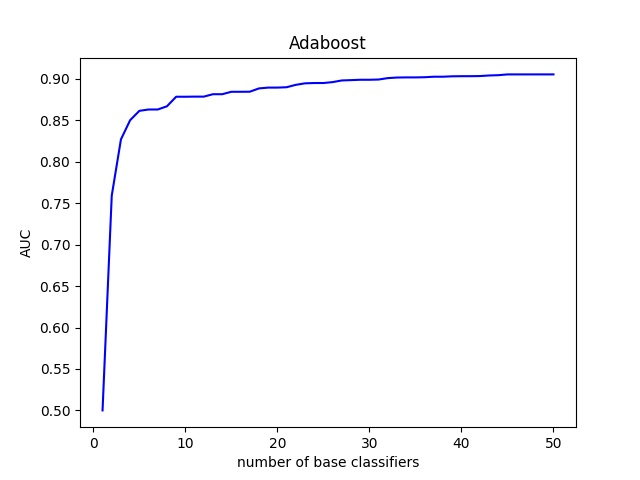
\includegraphics[scale=0.6]{Adaboost.jpg}}

        可以看出,当基学习器数量为25左右时,算法基本已经收敛不再有大的波动或增长。所以我取基学习器的数量为25,
        得到$AUC=0.897, accuracy=0.851$

    \subsubsection{RandomForest}
        随机森林算法的伪代码如下
        
        \begin{algorithm}  
            \caption{Random Forest算法}  
            \begin{algorithmic}[1] 
                \Require 训练集$D = \{ (\boldsymbol{x}_1, y_1), (\boldsymbol{x}_2, y_2), \cdots, (\boldsymbol{x}_m, y_m) \}$;
                        属性集$A = \{ a_1, a_2, \cdots, a_d \}$ ;
                        训练轮数$T$
                \Ensure 集成学习器$H(\boldsymbol{x})$
                \Function {RandomDecisionTree}{$D, A$} 
                    \State $node \gets $ create a tree node
                    \If {all samples in $D$ belongs to the same class $C$}
                    \State classify $node$ as class $C$
                    \EndIf
                    \If {$A = \emptyset$ \textbf{or} all samples in $D$ are equal on $A$}
                    \State classify $node$ as major class in $D$
                    \State \Return a tree with root $node$
                    \EndIf
                    \State $K \gets log_2 d$ features randomly chosen from $A$
                    \State $a_* \gets$ best feature chosen from $K$
                    \For {each value $a_*^v$ of $a_*$}
                    \State create a branch $node_l$ for $node$
                    \State $D_v \gets \{ (\boldsymbol{x}, y) \in D | x_{a_*}= a_*^v\}$
                    \If{$D_v=\emptyset$}
                    \State classify $node_l$ as major class in $D$
                    \State \Return a tree with root $node$
                    \Else
                    \State $node_l \gets $ \Call{RandomDecisionTree}{$D_v, K-\{a_*\}$}
                    \EndIf
                    \EndFor
                    \State \Return a tree with root $node$
                \EndFunction  
                \State  
                \Function{Train}{$D, A, T$}
                    \For{$i = 1, 2, \cdots, T$}
                        \State $S \gets$ samples randomly chosen from $D$ for $m$ times
                        \State $h_i \gets \Call {RandomDecisionTree}{S, A}$
                    \EndFor
                    \State \Return $H(\boldsymbol{x}) \gets \frac{1}{T} \sum_{i=1}^T h_i(\boldsymbol{x})$
                \EndFunction  
            \end{algorithmic}  
        \end{algorithm}
        数据预处理和5-Fold交叉验证的过程和AdaBoost完全相同,我这里就不再赘述。主要区别在于类RandomForest的实现。
        我设置了两个成员变量T、base,分别代表训练轮数、基学习器列表。
        除了三个成员函数train、predict和predict\_with\_prob之外,还有一个bootstrap\_sample函数用于自助采样每轮的训练数据。

        在bootstrap\_sample中,我自助采样每轮的训练数据,使用np.random.choice函数来从训练集中有放回地抽样m个数据,
        来训练决策树。这里我一次性将所有T组训练数据全部采样好,这个函数调用一次调用即可。

        在train中,我们先调用bootstrap\_sample获取T个学习器的训练数据,然后用这些训练数据训练T个决策树,都存入self.base中。

        在predict中,使用简单平均法,将T个基学习器的结果做平均,与0.5比较来得出是正类还是反类。

        在predict\_with\_prob中,流程与predict基本类似,区别在于不需要和0.5比较,直接返回概率即可。

        进行和AdaBoost一样的5-Fold交叉验证,得到的结果如图。

        {\centering
        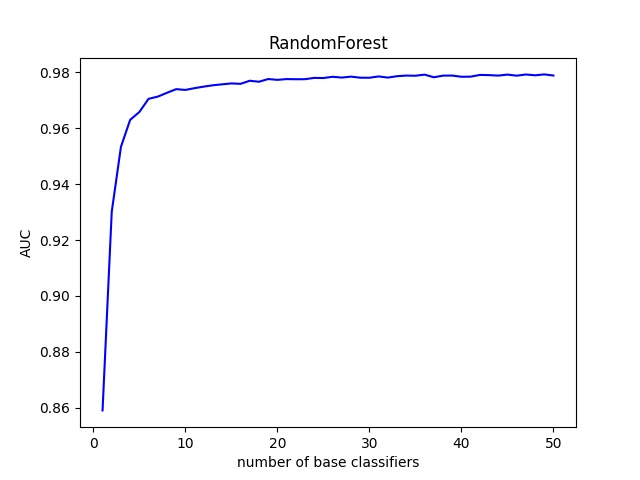
\includegraphics[scale=0.6]{RandomForest.jpg}}

        可以看出,当基学习器数量为15左右时,算法基本已经收敛不再有大的波动或增长。所以我取基学习器的数量为15,
        得到$AUC=0.880, accuracy=0.841$

    \subsection{实验感想}
        \begin{itemize}
            \item 
                为了体现集成学习对弱学习器的提升效果,我一开始将基学习器决策树的最大深度设为1,但是
                这样设置在RandomForest中效果很差,AdaBoost则相反。我经过查阅资料和思考,觉得这跟算法的目的有关。从偏差-方差
                的角度来看,AdaBoost主要是减小偏差,本身算法的设计就是为了减小与真实值的差距,所以基学习器弱一点是可以
                通过改变下一个学习器的分布来弥补的,而RandomForest是减小方差,是为了减小样本的不平衡造成的影响设计的,
                需要基学习器足够强,所以我对RandomForest没有设置深度限制,获得了较好的结果
            \item 
                基学习器数量对AUC的影响。可以从两个算法输出的折线图发现,虽然可能存在波动,但大体上AUC都是随基学习器的增多
                而变大的,且基学习器数量较少时增长块,基学习器数量较多时增长慢。要选择最优的数量,只需取趋近于收敛的点即可。
                数量较少时效果差,而数量较多时训练时间长。
            \item 
                对于AdaBoost中差错率为0的处理。其实这种情况一般不会发生,因为每个基学习器都是一个弱学习器。
                所以我设置为了直接返回。
            \item 
                AdaBoost中对于AUC的计算。计算AUC需要输出预测概率,而书上的AdaBoost算法是无法输出概率的。
                所以我对AdaBoost进行了改造,将所有的权重$\alpha_t$归一化到$[0, 1]$,就可以得到一个预测概率。
        \end{itemize}
		
\end{document}
